\section{Parcours différenciés}
\subsection{Parcours différenciés autour de la symétrie centrale}
\subsubsection*{Fiche d'exercice}\label{parcours_symetrie_centrale}
\begin{figure}[!h]
	\center{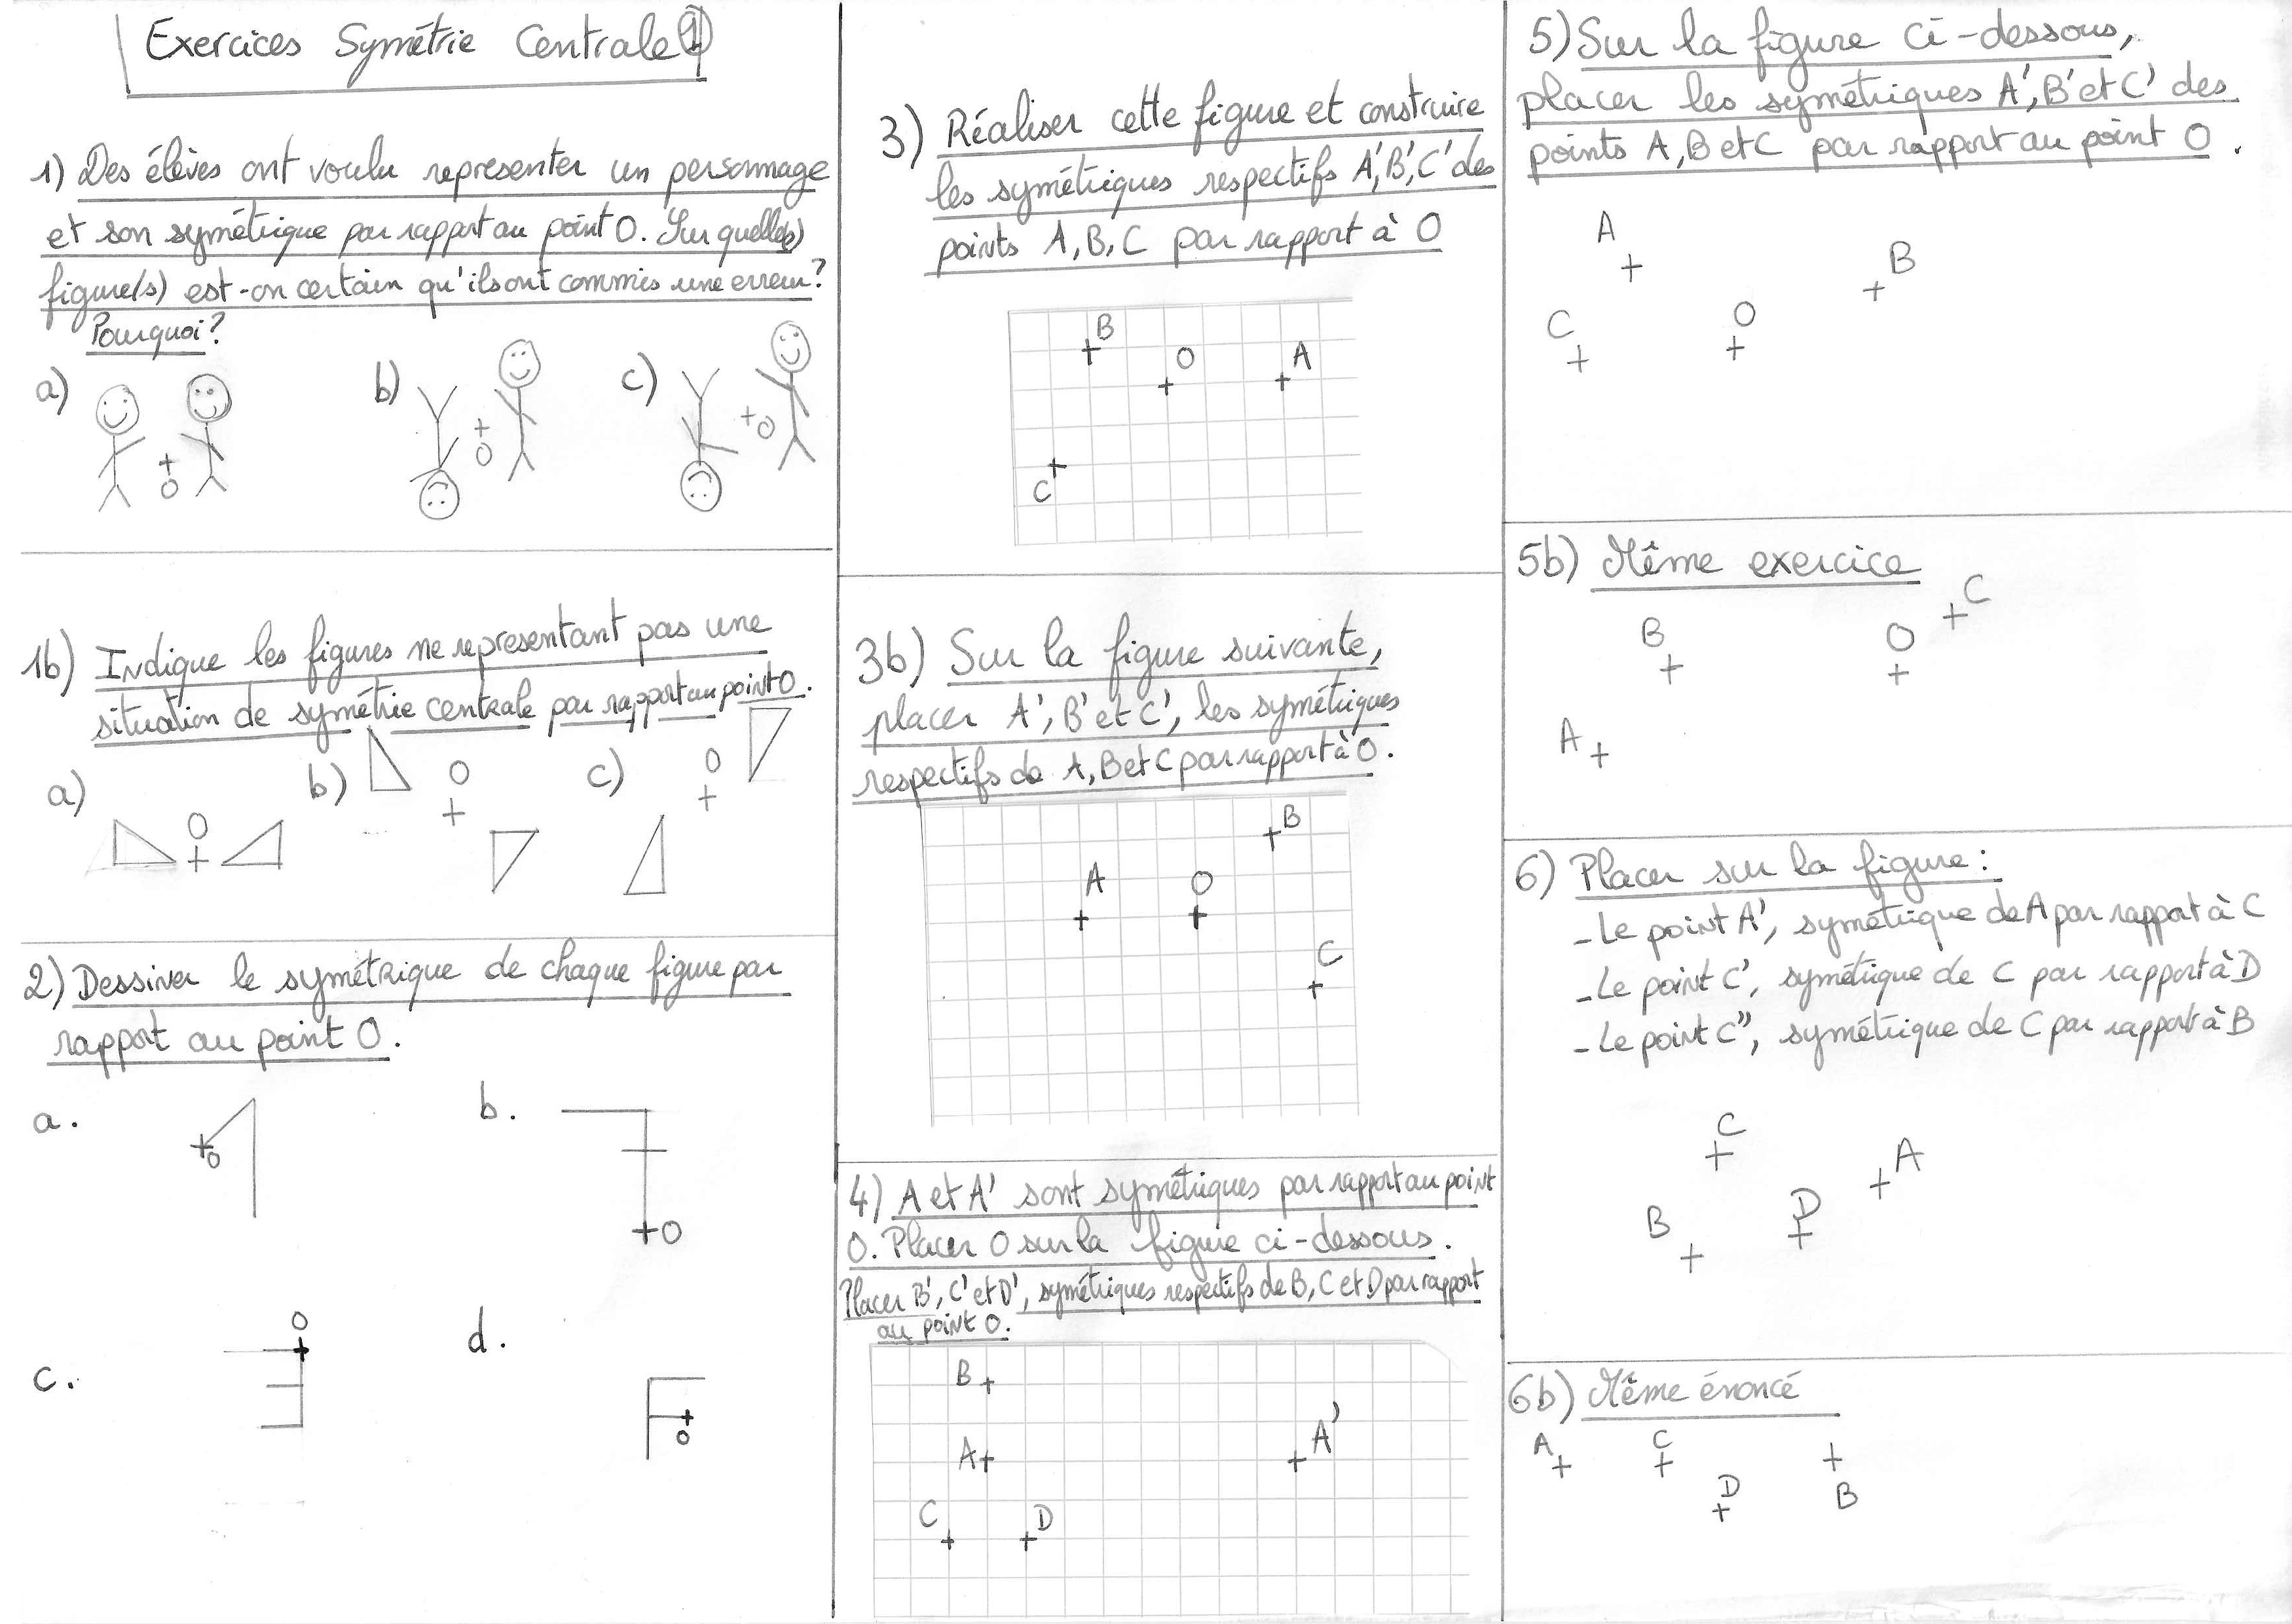
\includegraphics[scale=0.5]{img/Parcours_symetrie_julia.jpg}}
	\caption{Fiche d'exercices du parcours différencié}
\end{figure}
\subsubsection*{Parcours}
\begin{figure}[!h]
	\center{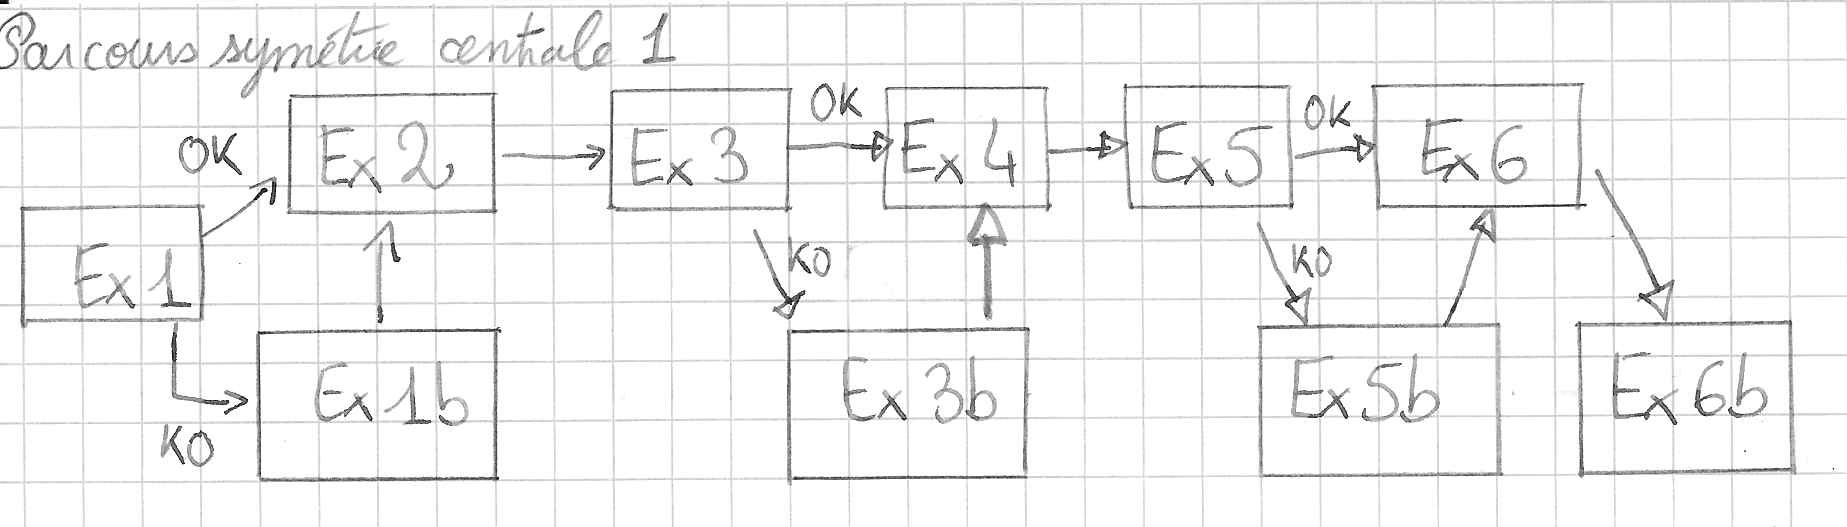
\includegraphics{img/Parcours_symetrie_julia2.jpg}}
	\caption{Parcours d'exercices à effectuer par les élèves}
\end{figure}
\subsubsection*{Productions d'élèves}\label{Prod_eleves_ju}
\paragraph{Parcours différencié : copies d'élèves de 5\up{ème} \\}
\begin{figure}[!h]
	\centering
	%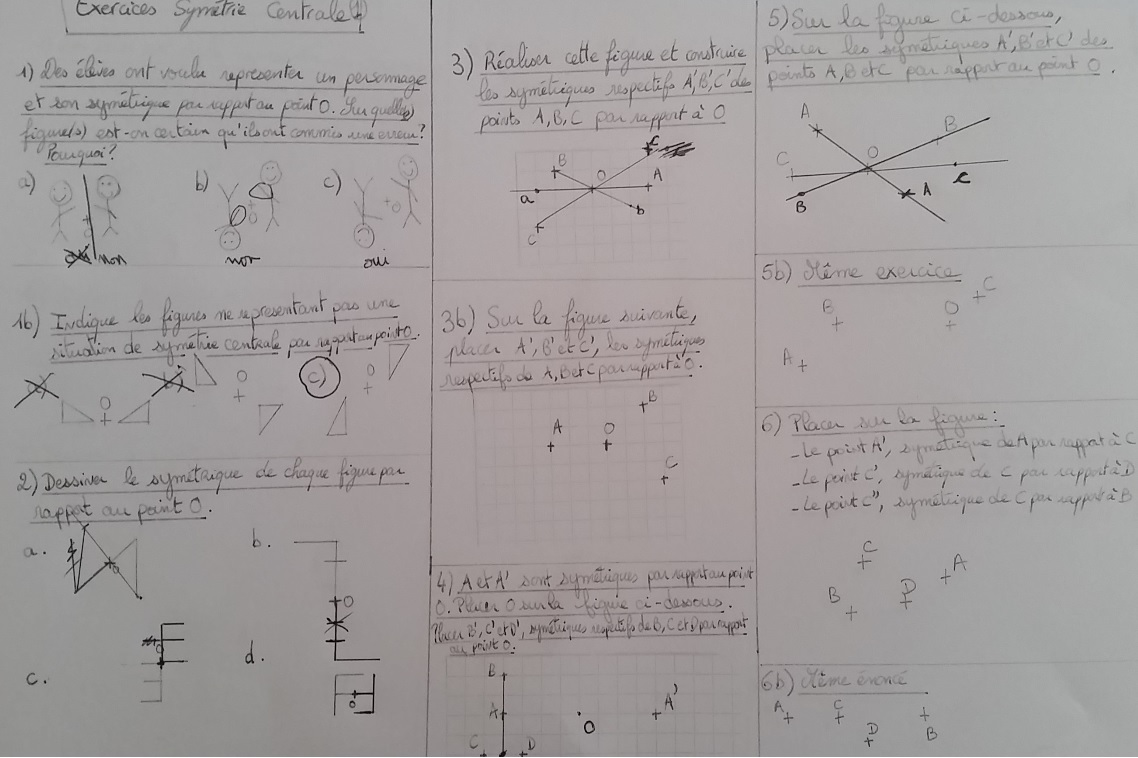
\includegraphics[scale=0.5]{img/symetrie_Ilyes.jpg}
	\caption{Parcours construction symétrie centrale d'Ilyès}
\end{figure}
\paragraph{}Ilyès est un élève en grande difficulté au premier trimestre, avec un comportement perturbateur (prise de parole, bavardages, pas de travail). Son comportement s'est fortement amélioré au second trimestre. Il fait partie du dispositif \textit{Fiche de suivi}, ce qui a probablement eu un impact important sur son travail. Mes collègues m'indiquent cependant qu'ils ne remarquent pas des progrès aussi importants dans leurs matières, notamment sur la capacité à travailler en autonomie.\\
Pour le parcours de construction par symétrie centrale, Ilyès a mis du temps à se mettre au travail mais a fait les efforts nécessaires pour tenter de construire les figures demandées. Il a notamment fait de nombreux aller-retour vers les corrections et n'a pas hésité à poser des questions précises sur les méthodes de constructions. C'est pour cela que l'on observe des ratures et des traits de construction approximatifs. J'ai du lui dire qu'un écart d'un millimètre n'était pas très important mais que l'alignement des points l'était plus par exemple. 
\begin{figure}[!h]
	\centering
	%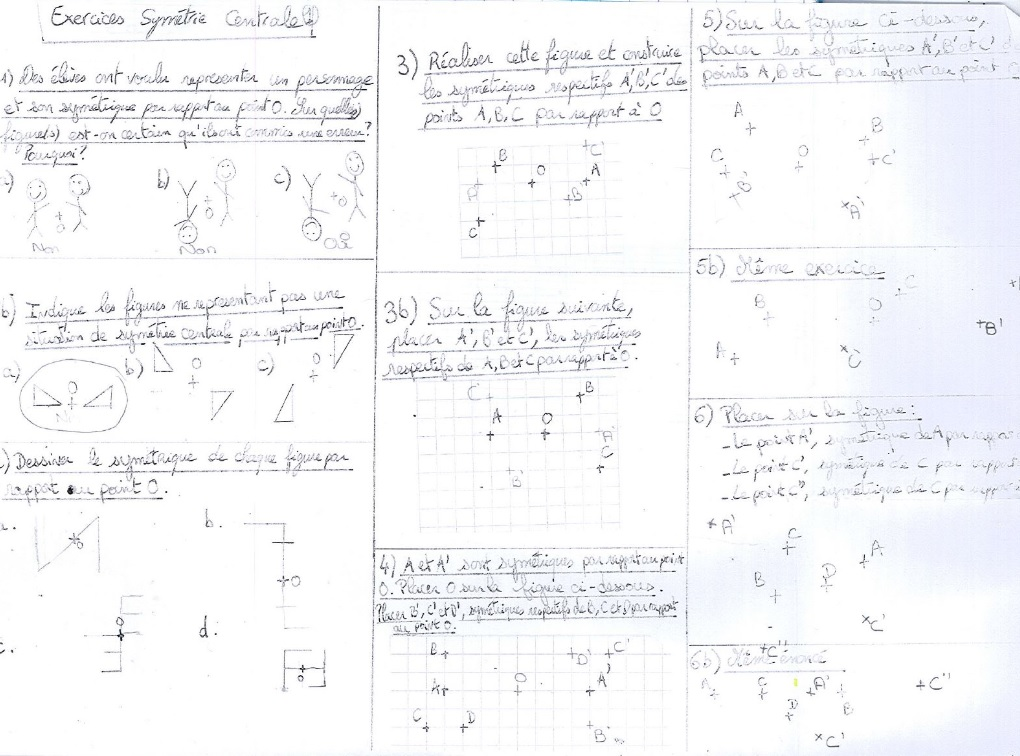
\includegraphics[scale=0.4]{img/symetrie_Dahlia.jpg}
	\caption{Parcours construction symétrie centrale de Dahlia}
\end{figure}
\paragraph{}Dahlia est une élève à fort caractère qui a besoin d'attention face aux difficultés. Il s'agit cependant d'une élève plus à l'aise en mathématiques que la plupart de ses camarades. Suite à l'instauration des parcours différenciés, elle a gagné en autonomie mais continue de se braquer si elle n'obtient pas une aide du professeur. En revanche, elle a adopté le rôle de tuteur pour deux élèves en difficultés et a améliorer son expression orale. Il s'agit d'une des élèves qui m'ont convaincue de mettre en place d'autres supports de différenciation, notamment pour débloquer les élèves.\\
Come le montre la résolution de son parcours différencié, Dahlia n'a pas de difficulté dans la construction de figures par symétrie centrale. Elle a cependant eu besoin d'être recadrée à plusieurs reprises et d'être rassurée dans son travail.
\paragraph{Evaluation sommative symétrie centrale : copies d'élèves de 5\up{ème}\\}
Les progrès d'Ilyès dans cette évaluation sont flagrants, on observe bien que les constructions sont plus précises et plus « \textit{propres} ». Ilyès, comme Dahlia, n'a pas demandé d'aide ou de confirmation de son travail lors du contrôle. Ces deux élèves ont visiblement gagné confiance en eux sur cette séquence (comme observé lors des questions à l'oral). Les compétences demandées sont de plus acquises.
\begin{figure}[!h]
	\centering
	\subfloat{{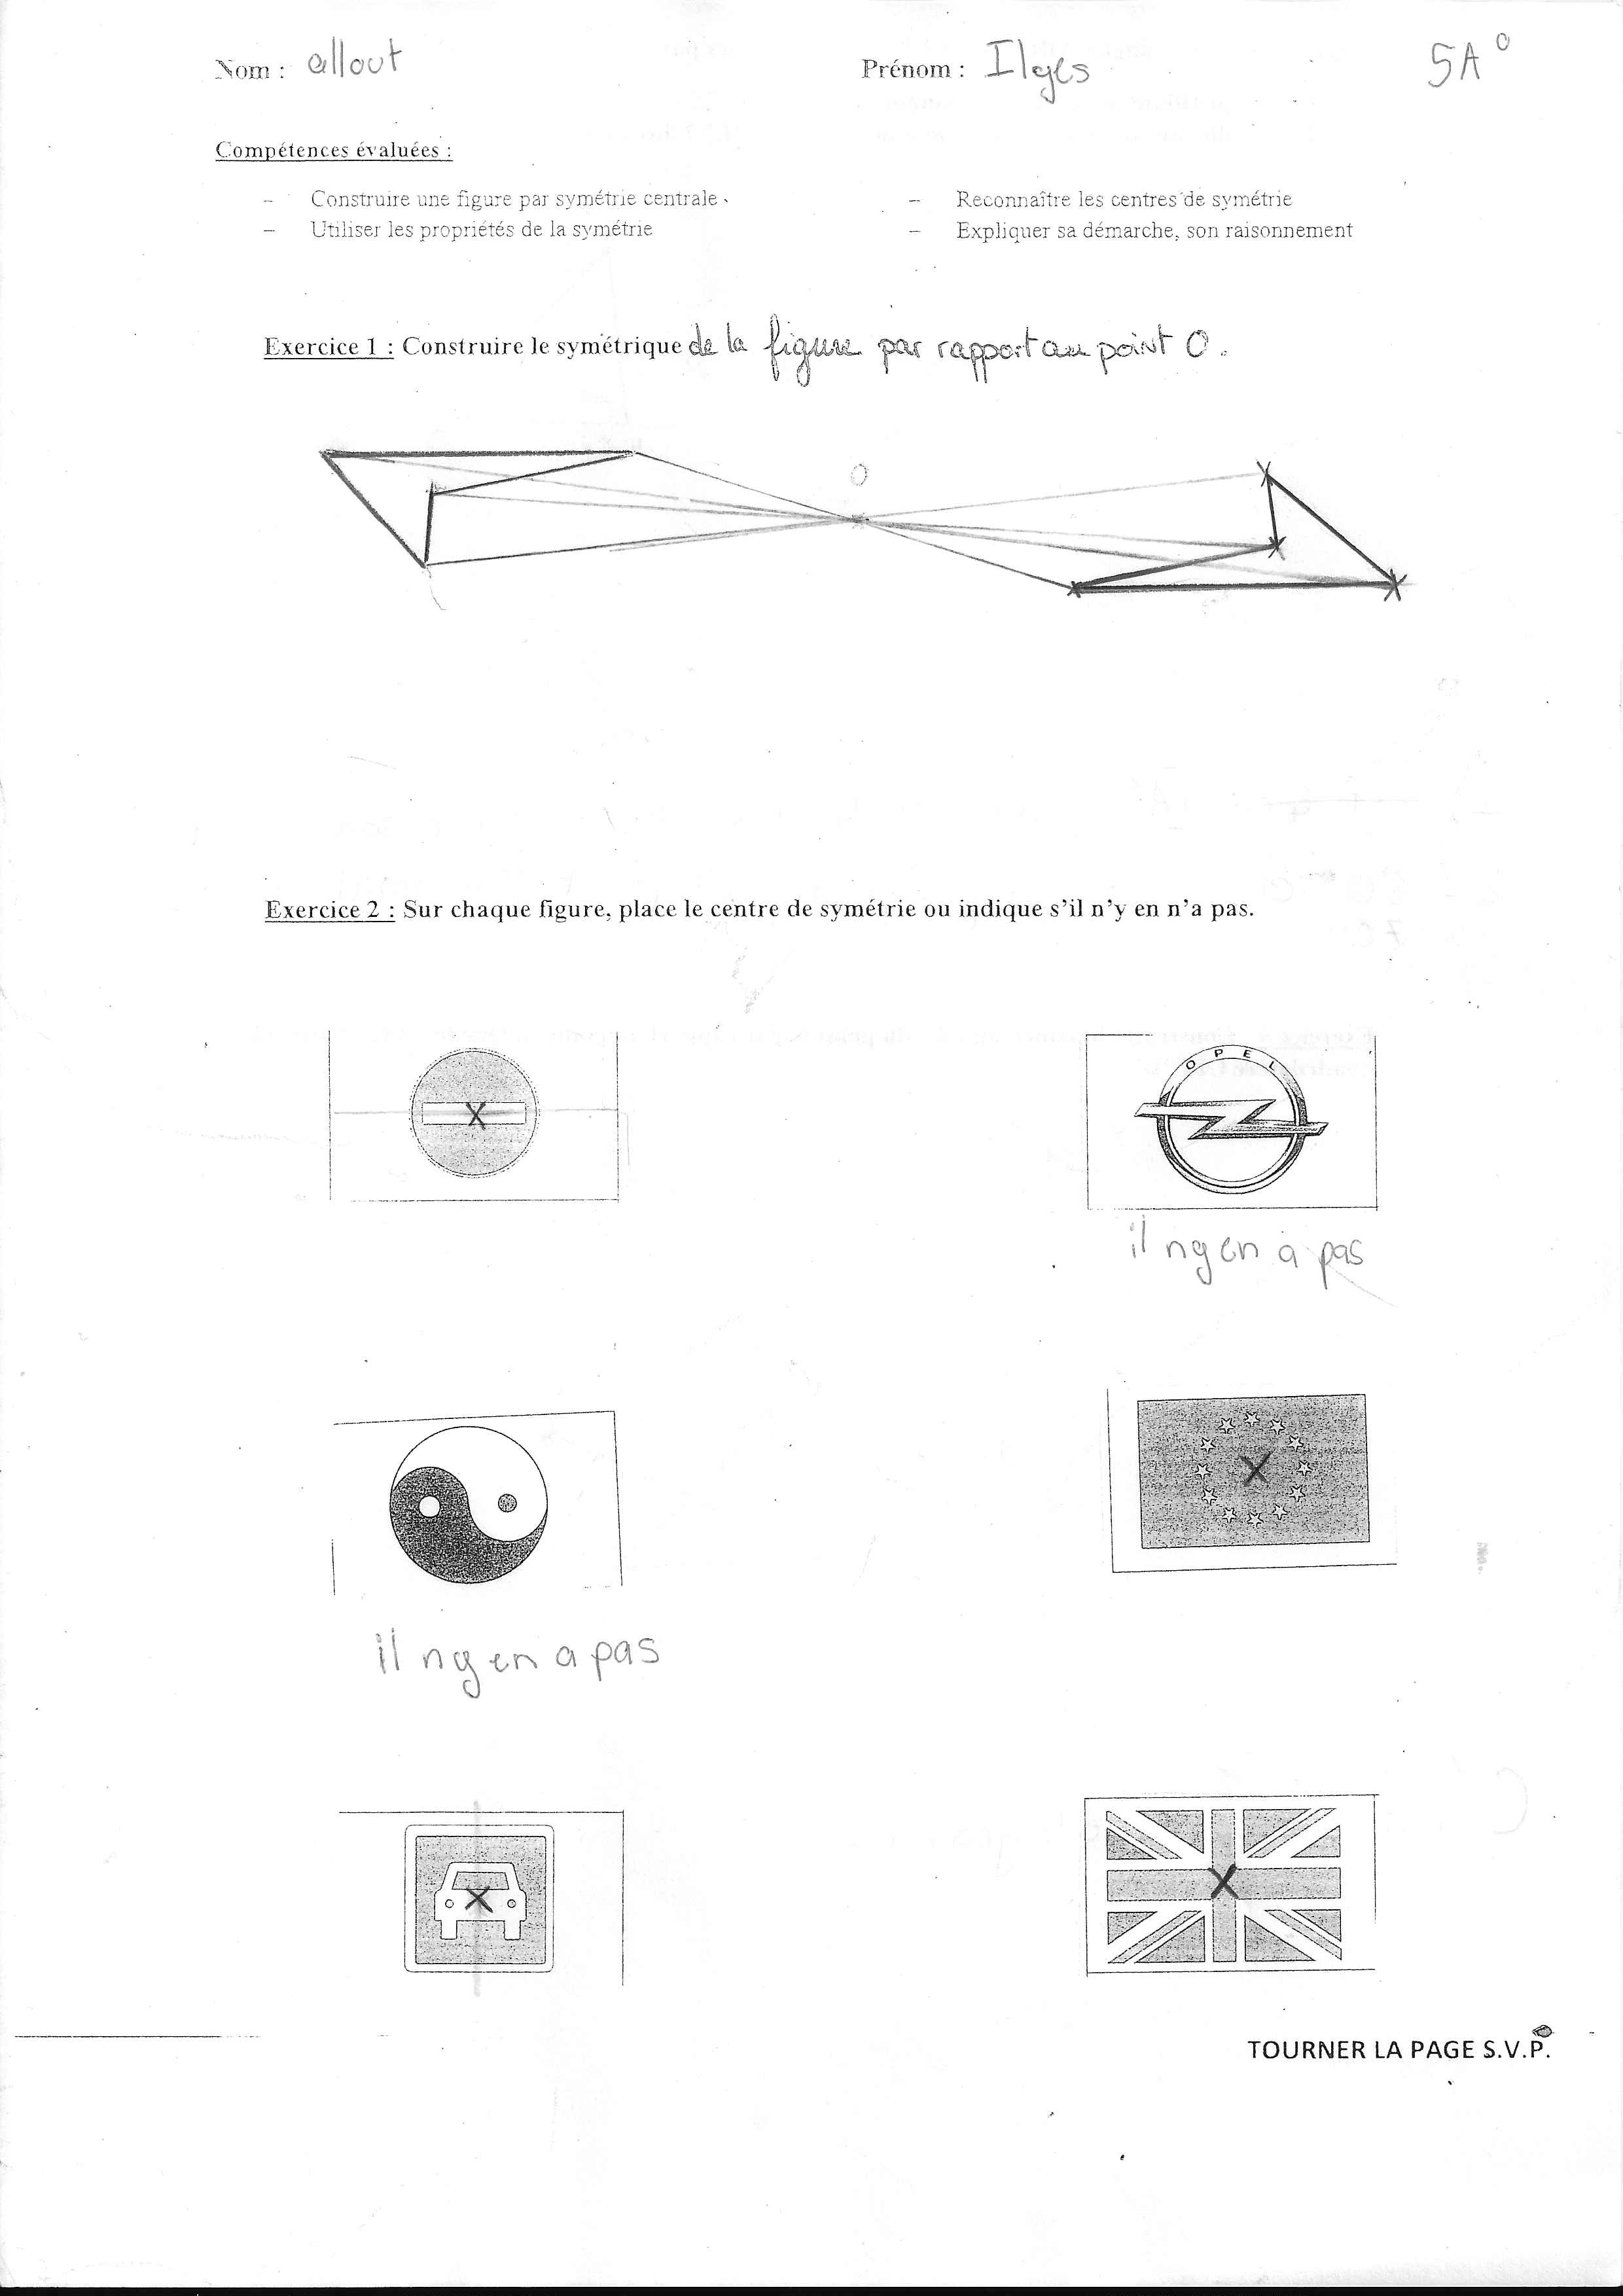
\includegraphics[scale=0.25]{img/Ilyes1.jpg}}}
	\qquad
	\subfloat{{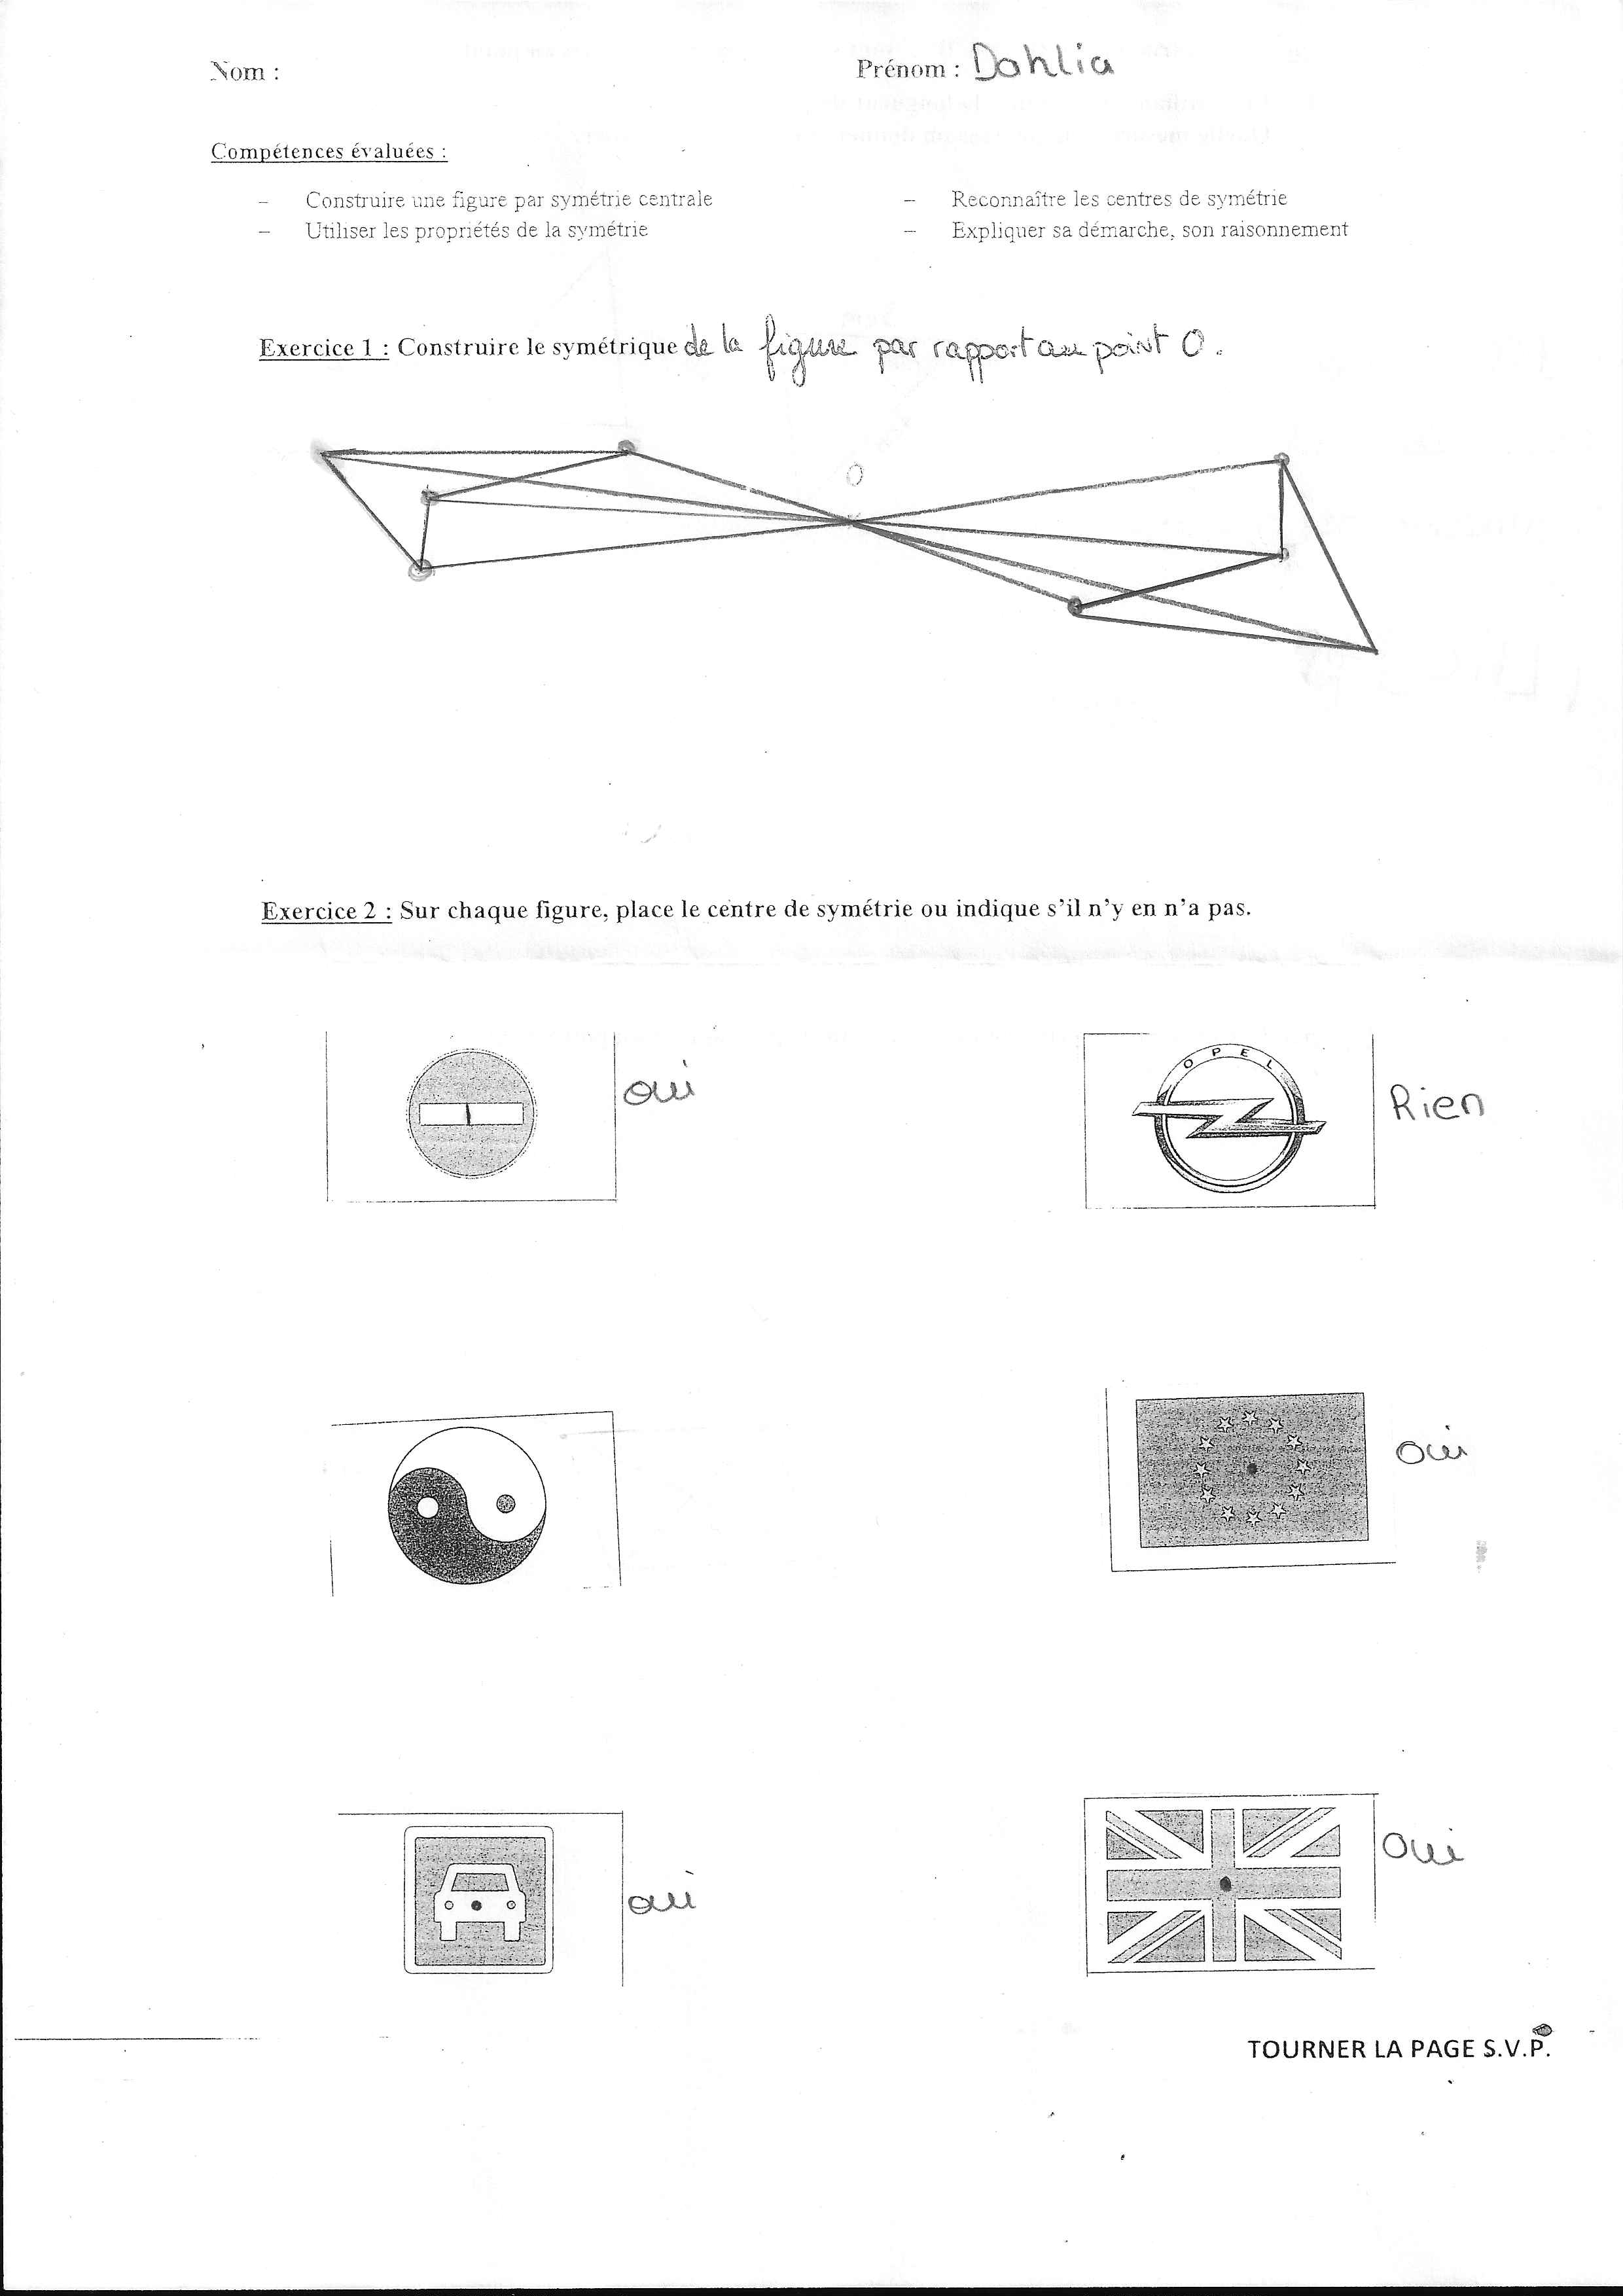
\includegraphics[scale=0.25]{img/Dahlia1.jpg}}}
	\caption{Evaluation d'Ilyes et de Dahlia}
	\label{fig:Eval_symetrie}
\end{figure}

